\chapter{Introduction}
\pagenumbering{arabic}

%%%%%%%%%%%%%%%%%%%%%%%%%%%%%%%%%%%%%%%%%%%%%%%%%%%%%%%%%%%%%%%%%%%%%%%%%%%%%%%%%%%%%%%%%%%%%%%%%%%%

\section{Objectives}

The primary objective of this project was to evaluate the usefulness of the Robot Operating System (ROS) \cite{ros_site} as a framework for developing complex robotic systems. Specifically, we looked to explore a range of standard and community-provided packages available for use with ROS. These packages provide a large variety of functionalities, including device drivers for particular sets of sensors, simulation environments, and full autonomous navigation suites.

As a secondary objective, we aimed to evaluate the usefulness of open-source software as a means for accelerating development of these complex systems. Additionally, by using this open-source software in the project, we set out to contribute in-kind by making any developments open-source.

%%%%%%%%%%%%%%%%%%%%%%%%%%%%%%%%%%%%%%%%%%%%%%%%%%%%%%%%%%%%%%%%%%%%%%%%%%%%%%%%%%%%%%%%%%%%%%%%%%%%

\section{Achievements}
Through the use of ROS, we show that it was indeed possible to implement complex behaviours, such as environment mapping and autonomous navigation, achieved with relative simplicity. Almost all functionality for these behaviours were provided by these standard and community-provided packages. In particular, the robot can walk, detect and interpret the environment surrounding it, and navigate around that environment while avoiding any obstacles.

\begin{figure}[!h]
    \centering
    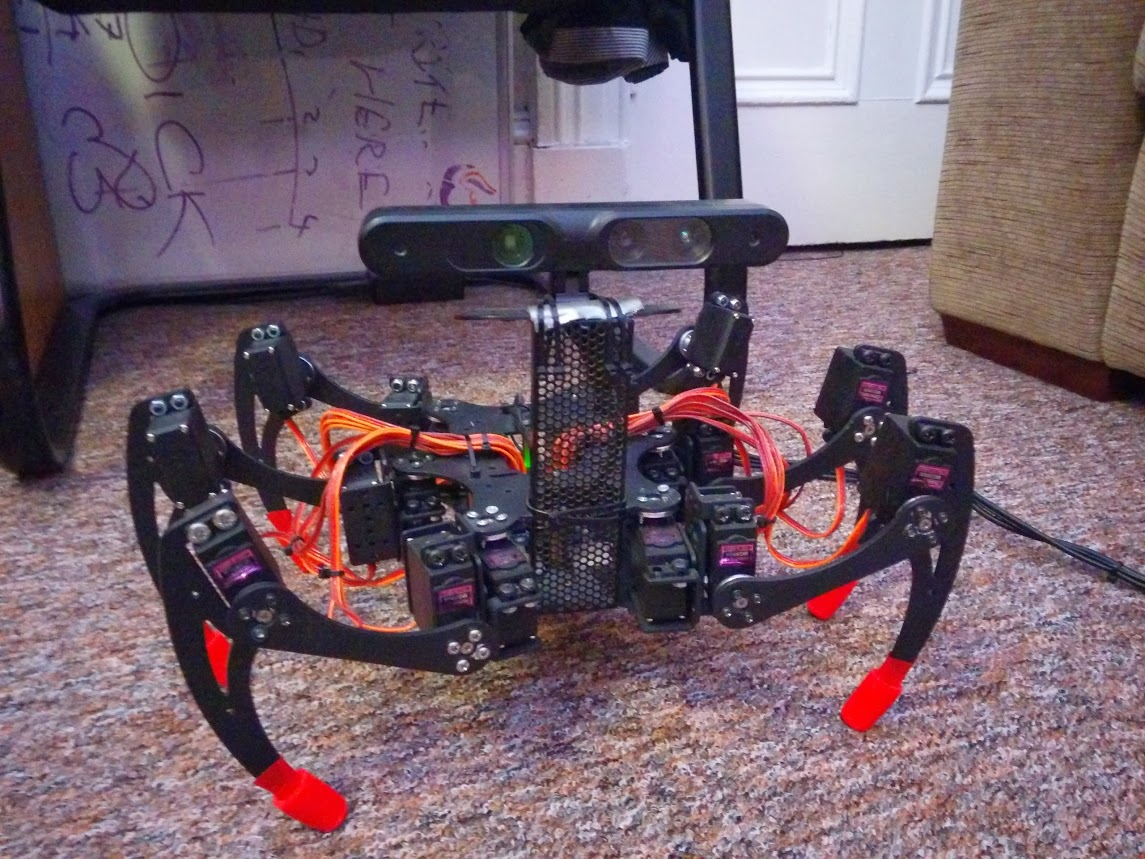
\includegraphics[width=12cm]{hexapod_body1}
    \caption{This hexapod is the target hardware platform for this project.}
\end{figure}

Furthermore, we show that non-standard hardware, such as the robot used throughout this project, can be integrated into a ROS-based system with relative ease. Most examples of robots using this framework tend to move themselves using either wheels or tracks, but in this case a walker-style robot is used.

%%%%%%%%%%%%%%%%%%%%%%%%%%%%%%%%%%%%%%%%%%%%%%%%%%%%%%%%%%%%%%%%%%%%%%%%%%%%%%%%%%%%%%%%%%%%%%%%%%%%

\section{Ramifications}